\newpage
\subsection{calibrate}
The calibrate functions go through a procedure that return correct correction and conversion factors. These should afterwards be stored in the metadata, category `conversion factors'. 

\paragraph{TOF $\rightarrow m/q$ factor}

\paragraph{detection center position}

\paragraph{detector rotation}

\paragraph{residual momentum minimualization}
The residual momentum of a two-body process, resulting in two cations, can be used to calibrate the spectrometer. This module minimizes the relative norm of the residual momentum:

\begin{align}
f_{min} = \frac{norm(\vec{p}_{res})}{norm(\vec{p}_{1} - \vec{p}_{2})} = \frac{norm(\vec{p}_{1} + \vec{p}_{2})}{norm(\vec{p}_{1} - \vec{p}_{2})}
\end{align}

The variables that are tweaked during this optimization:

\begin{itemize}
\item corr.det1.dX	(X-shift of the raw image)
\item corr.det1.dY (Y-shift of the raw image)
\item spec.volt.Ve2s (voltage of grid between electron MCP and source ('pusher'))
\item conv.det1.TOF\_2\_M2Q.factor (Conversion factor from mass 2 charge to TOF) 
\item conv.det1.TOF\_2\_M2Q.t0 (time correction)
\end{itemize}

This function requires the input values to be roughly calibrated, so should be used as a final calibration: the solver only searches in a small solution domain and only a local minimum is found. 

\begin{figure}[H]
   \centering
    \centerline{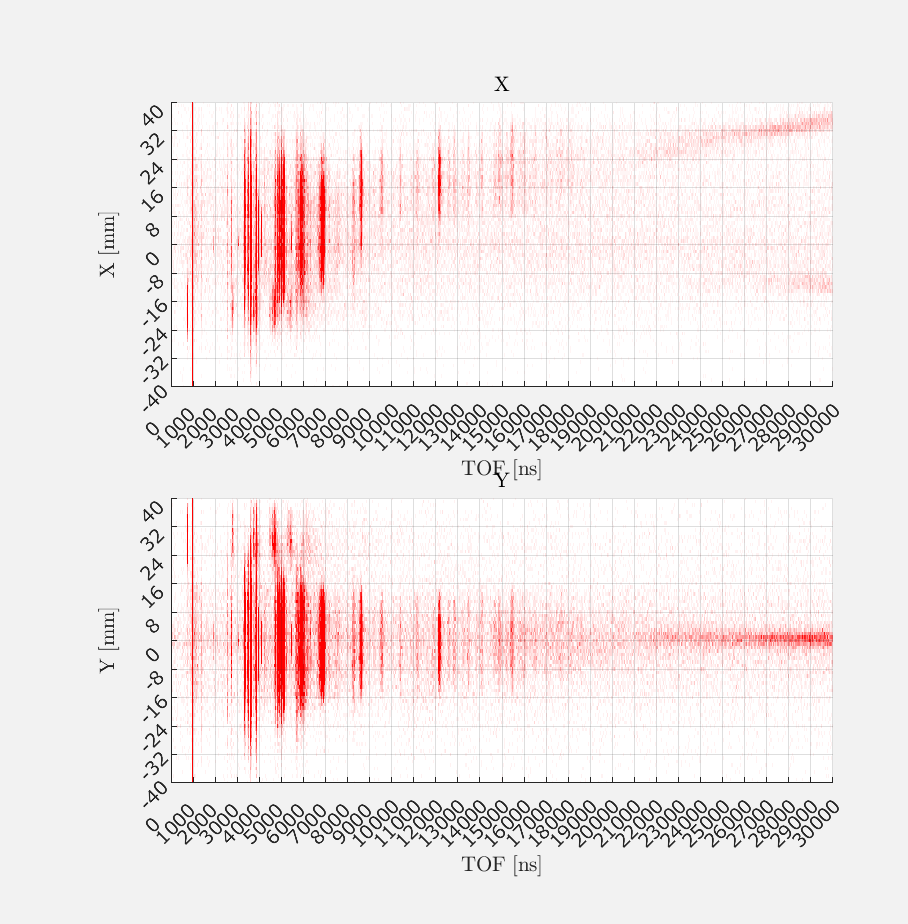
\includegraphics[width=0.9\textwidth]{Graphics/MB_calib.png}}
\caption{Example of a molecular beam calibration}
\label{MB_calib}
\end{figure}
